\section{Two Parallelization Regimes for Lookahead Construction}
\begin{figure}[t]
\centering
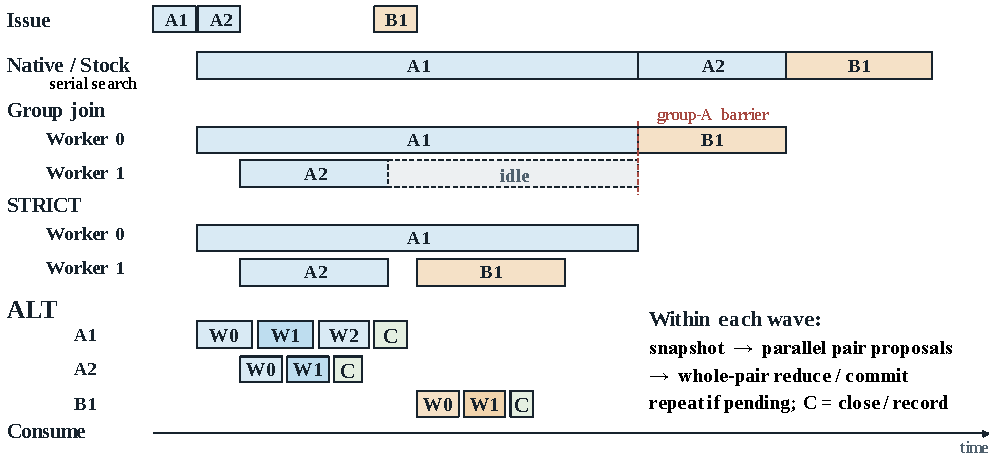
\includegraphics[width=\columnwidth]{figures/timeline.pdf}
\caption{Illustrative schedules for samples $A_1,A_2,B_1$. Group waits at the group boundary. STRICT can issue $B_1$ while $A_1$ is active and still consume in native order. Within an ALT sample, $W_i$ denotes a wave and C marks bucket closure.}\label{fig:contracts}
\end{figure}
\begin{figure*}[t]
\centering
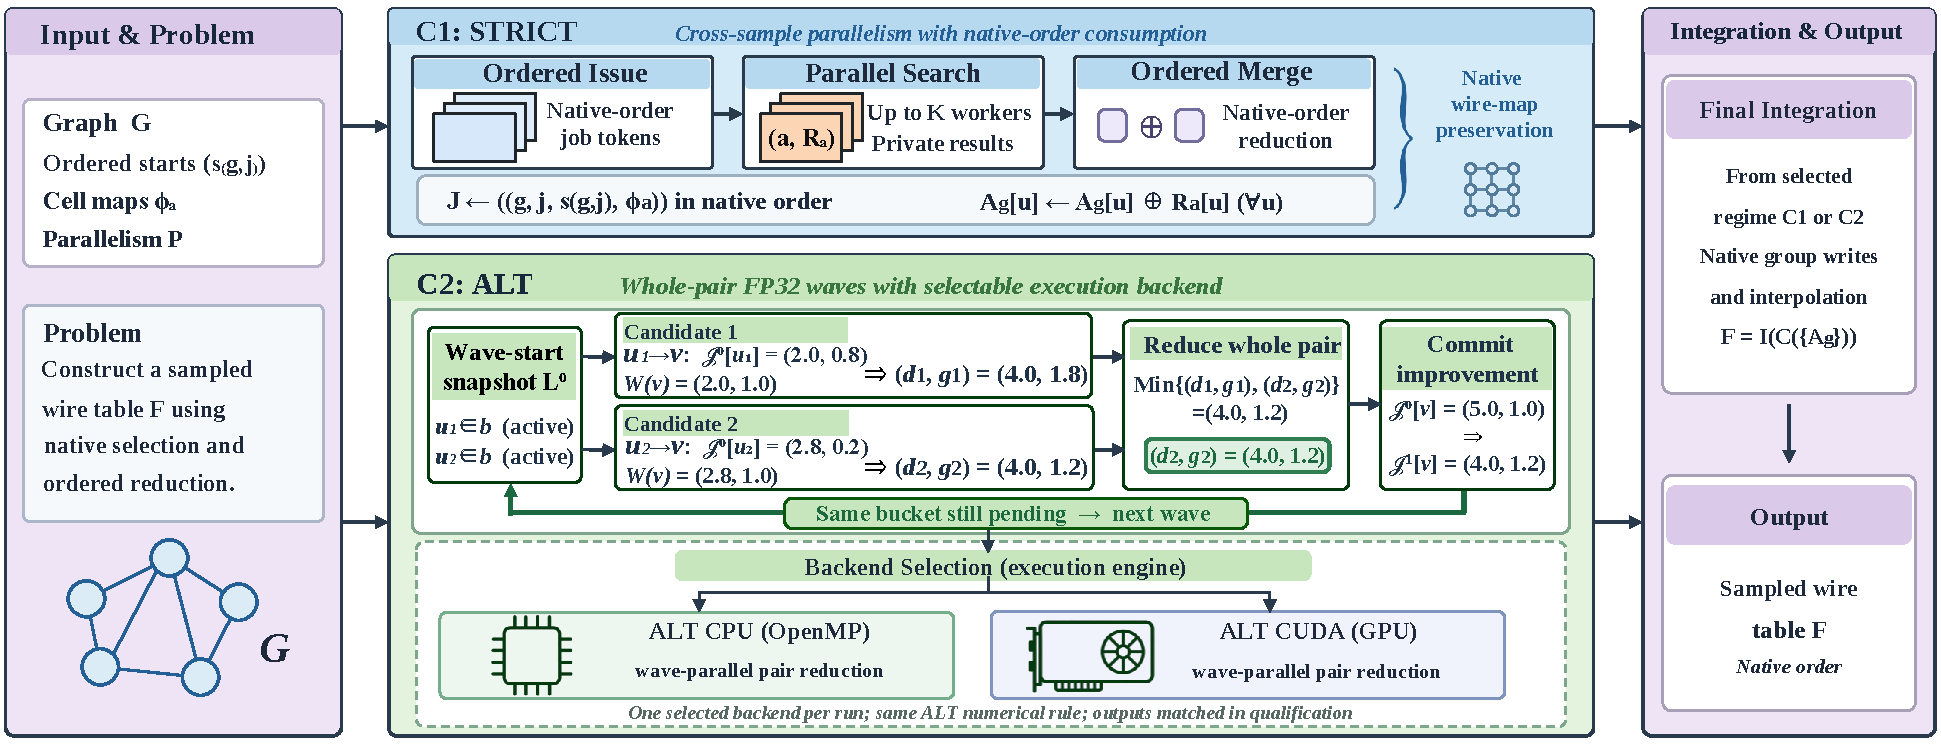
\includegraphics[width=\textwidth]{figures/framework.pdf}
\caption{Layer-aware lookahead construction. In C1, $P$ counts workers and $K$ bounds live tokens. Proposition~\ref{prop:strict} gives the native-map guarantee. C2 distributes samples across CPU workers or processes active nodes in parallel on the GPU (CUDA), using the same whole-pair rule. The selected regime returns sample results for native group writes and interpolation.}\label{fig:framework}
\end{figure*}

Figure~\ref{fig:contracts} compares schedules. Figure~\ref{fig:framework} follows a batch from its ordered starts to the native wire table.
\subsection{C1: Private Samples and Ordered Consumption}
In Algorithm~\ref{alg:c1}, token $a$ identifies the group, ordinal, source and cell map across group boundaries. Worker $p$ resets its private queue, visited costs and expanded bits in $S_p$. Its flood reads the shared graph with native geometry, edge eligibility and arithmetic.

\begin{algorithm}[t]\footnotesize
\caption{Bounded STRICT sample pipeline (C1)}\label{alg:c1}
\Input{Graph $G$, ordered starts $(s_{g,j})$, cell maps $\phi_a$, parallelism $P$}
\Output{Sampled wire table $F$}
$\mathcal J\gets\langle(g,j,s_{g,j},\phi_a)\rangle_{(g,j)\text{ in native order}}$\;
$K\gets\min(|\mathcal J|,\max(1,2P)),\quad A_g[\cdot]\gets\bot\quad(\forall g)$\;
\Stage{\textsc{Issue}$()$}{
  \Return $\operatorname{NextIndex}(\mathcal J)$\;
}
\Stage{\textsc{Search}$(a)$}{
  $S_p\gets\operatorname{Reset}(S_p)$\;
  $R_a\gets\operatorname{NativeFlood}(G,s_a,\phi_a,S_p)$\;
  \Return $(a,R_a)$\;
}
\Stage{\textsc{Merge}$(a,R_a)$}{
  $A_{g(a)}[u]\gets A_{g(a)}[u]\oplus R_a[u]\quad(\forall u)$\;
}
$\operatorname{Pipeline}_K(\textsc{Issue},\textsc{Search},\textsc{Merge})$\;
\Return $\mathcal I(\mathcal C(\{A_g\}))$\;
\end{algorithm}

A result retains its token until the consumer applies $\oplus$ in issue order. At most $K$ tokens are live. Native writes and fills follow the join. Flat retains all $J$ results until reduction. Group joins after each group.

\begin{proposition}\label{prop:strict}
Assume native sample selection, contexts, visitation, arithmetic, occupancy, commit and interpolation. For finite occupied delays, private floods and original-order strict-delay reduction reproduce the native wire table.
\end{proposition}
\noindent\textbf{\emph{Proof.}} Each private flood produces the same per-cell representative as its native execution. For an occupied cell, ordered reduction selects the least delay and retains its earliest sample on equal delay:
\begin{equation}
 a^*(g,u)=\arg\min_{a:g(a)=g,\ R_a[u]\ne\bot}(R_a[u].d,a).
\end{equation}
The implementation uses the native missing-state predicate and insertion, not a generic tuple sort. Occupancy and associated congestion therefore agree cell by cell. Identical group writes and interpolation preserve this agreement. Completion order never enters the reduction. $\square$

Changing heap ties, exceptional-value handling or recording geometry violates the premises. The proposition is about wire maps, not route trajectories. ALT below changes the sample engine and does not inherit this proof.

\subsection{C1 Work, Width and Storage}
Let $t_a$ include sample reset, traversal and recording, and $W_g=\sum_{a:g(a)=g}t_a$. Ignoring launch, merge and interference, ideal search schedules obey
\begin{align}
 T_{\rm group}&\geq\sum_g\max\{W_g/P,\max_{a:g(a)=g}t_a\},\\
 T_{\rm global}&\geq\max\{\textstyle\sum_a t_a/P,\max_a t_a\}.
\end{align}
An early slow sample can stall ordered consumption and occupy tokens. For private workspace $S(N)$ including the queue, Pipeline needs $O(P S(N)+KC+|\mathcal G|C+J)$ storage beyond the shared graph. Flat replaces $KC$ with $JC$. Dense reduction visits $O(JC)$ cells, in addition to enumeration, writes and interpolation. Flood work depends on queue traffic, termination and reset.

\subsection{C2: Whole-Pair FP32 Waves}
ALT\_BUCKET\_FP32\_V1 makes the inner ordering rule explicit. A node label $L[v]=(d,q)$ is compared lexicographically:
\begin{equation}
 a\prec b\ \Longleftrightarrow\ a_d<b_d\ \lor\ (a_d=b_d\land a_q<b_q).
\end{equation}
Both coordinates come from one predecessor label plus the destination cost. Native insertion compares delay alone. ALT initializes the source to $(0,0)$, other labels to an infinity sentinel and output cells to missing.

The scheduling key $B(d)=\mathrm{bits}_{32}(d)\gg h$ uses exact delay bits at shift $h=0$. Shift 20, used for native ALT timing, groups delays without quantizing stored labels. Costs and candidates must be positive normal FP32 or positive zero. Admission checks inter-cluster non-SINK node costs, and expansion checks each accumulated pair. Infinity marks unreached nodes internally. ALT CPU uses round-to-nearest with contraction and fast math disabled. ALT GPU uses explicit round-to-nearest CUDA addition.

In Algorithm~\ref{alg:c2}, $T_a$ contains the distinct mapped target cells. $\operatorname{Pop}$ removes bucket $b$ from directory $\mathcal D$; only entries whose current key $\pi[u]=b$ are active. $\operatorname{Publish}$ schedules a new key and suppresses duplicate current notifications. ALT CPU filters stale directory entries. ALT GPU replaces the pending key directly.

\begin{algorithm}[t]\footnotesize
\caption{Whole-pair FP32 waves (C2)}\label{alg:c2}
\Input{$G$, source $s_a$, cell map $\phi_a$, targets $T_a$, key $B$}
\Output{Sample map $R_a$}
$R_a[\cdot]\gets\bot,\quad L[\cdot]\gets(+\infty,+\infty)$\;
\lIf{$T_a=\varnothing$}{\Return $R_a$}
$\pi[\cdot]\gets\bot,\quad\mathcal D,\mathcal H\gets\varnothing,\quad L[s_a]\gets(0,0)$\;
$\operatorname{Publish}(\mathcal D,\pi,s_a,0)$\;
\While{$\mathcal D\ne\varnothing$}{
  $b\gets\min\operatorname{keys}(\mathcal D),\quad X\gets\operatorname{Pop}(\mathcal D,b)$\;
  $U\gets\{u\in X:\pi[u]=b\},\quad \mathcal H\gets\mathcal H\cup U$\;
  $\pi[U]\gets\bot,\quad L^0\gets L,\quad Q\gets L^0$\;
  \ForEach{$u\in U,\;v\in\Gamma(u)$}{
    $z\gets\operatorname{RN}_{32}(L^0[u]+w(v))$\;
    $Q[v]\gets\min_{\prec}(Q[v],z)$\;
  }
  \ForEach{$v$ with $Q[v]\prec L^0[v]$}{
    $L[v]\gets Q[v]$\;
    $\operatorname{Publish}(\mathcal D,\pi,v,B(L[v].d))$\;
  }
  \If{$b\ne\min\operatorname{keys}(\mathcal D)$}{
    \ForEach{$v\in\mathcal H$ with $c=\phi_a(v)\ne\bot$}{
      $R_a[c]\gets\min_{\prec}^{\bot}(R_a[c],L[v])$\;
    }
    $\mathcal H\gets\varnothing$\;
    \lIf{$\operatorname{dom}(R_a)=T_a$}{\Return $R_a$}
  }
}
\Return $R_a$\;
\end{algorithm}

$\Gamma(u)$ lists eligible neighbors in native order, including the SINK stopping rule. $\operatorname{RN}_{32}$ rounds each coordinate; $\min_{\prec}$ selects a whole pair. All proposals read the committed labels $L^0$ before any improvement is published. The snapshot and $Q\gets L^0$ are logical: ALT CPU initializes each proposal on first touch, while ALT GPU carries forward proposals equal to the committed labels.

Clearing $\pi[U]$ allows same-bucket improvements to enter the next wave. $\mathcal H$ collects expanded nodes until the bucket closes, taking $\min\varnothing=+\infty$. At closure, $\min_{\prec}^{\bot}$ accepts a first mapped IPIN pair in a missing cell and otherwise keeps the smaller pair. $\operatorname{dom}(R_a)$ contains occupied cells; exhaustion leaves unreachable cells missing. Invalid numerics or exceeded guards abort without partial output. FP32 rounding can collapse distinct delays and change which congestion tie survives.

\subsection{CPU/GPU Mapping and Costs}
ALT CPU takes the full native job list. An OpenMP dynamic loop distributes samples across workers, each with private scratch arrays and a sparse ordered map of pending buckets. ALT GPU allocates all $J$ samples together. Grid dimension $y$ selects a sample, while $x$ and 256-thread blocks select nodes. Each active node thread scans its own adjacency.

For admitted nonnegative floats the unsigned key
\begin{equation}
 H(d,q)=(\mathrm{uint64}(\mathrm{bits}_{32}(d))\ll32)
          \mathbin{|}\mathrm{bits}_{32}(q)
\end{equation}
orders complete pairs. The GPU backend uses a 64-bit atomic minimum on each destination proposal; collisions select one actual candidate pair. Separate expansion, commit/minimum-scan, confirmation and advance kernels provide wave boundaries. The commit scan reduces pending keys within each block before one atomic minimum per block; confirmation records IPIN pairs only at closure. Advance scans output occupancy per sample. A host completion-count copy waits each batch round, followed by device synchronization and full output readback/unpacking. The contexts field configures CPU workers; it does not measure GPU occupancy.

Let $A_{a,k}$ be active nodes, $E_{a,k}$ actually inspected adjacency entries (including rejected edges), $U_{a,k}$ touched destinations and $D_{a,k}$ directory operations in wave $k$. CPU work includes initialization $O(J(N+C))$, $\sum_{a,k}(|A_{a,k}|+|E_{a,k}|+|U_{a,k}|)$, stale-entry filtering, closed-set recording and ordered-directory costs $O(\sum_{a,k}D_{a,k}\log(1+B_{a,k}))$, where $B_{a,k}$ is the number of live directory buckets. Repeated waves can inspect an edge many times. GPU work additionally includes dense scans over allocated $JN$ slots each batch round and closure output scans; for $W$ rounds a useful accounting is
\begin{equation}
 O\!\left(J(N+C)+WJN+\sum_{a,k}|E_{a,k}|+\sum_a H_a C\right),
\end{equation}
where $H_a$ counts closure occupancy scans. Atomic contention, launches and host waits affect elapsed time beyond this work count. Neither formula assumes a single visit per edge.

For the GPU representation, arrays require $25JN+8JC$ bytes for labels/proposals, pending, closed flags, mapping and output, plus $8(N+1)+16N+8M$ for CSR/nodes/edges and cost/job metadata. Admission estimates the complete allocation and requires it to fit within 80\% of free device memory; allocation/API errors remain failures. Native ABI shape checks and finite wave/time guards further bound execution. An auxiliary qualification on the full 9,595,752-node GEMM graph admitted all 40 samples and verified outputs and routes.

The host exports graph costs and sample geometry, calls one backend and merges results in native order. \constructiontime{} includes conversion, allocation, transfer, synchronization, handoff and native writes/interpolation.
